% !TeX root = ../thesis.tex

\chapter{针对处理器系统的攻击}{Attacks on Processor Systems}
本章将基于SiFive公司的HiFive Unmatched SoC平台实现一种针对处理器系统的
基于PCIe DMA的非授权访问攻击。使用这种手段,攻击者可以操纵专门设计的硬件
或通用硬件(例如GPU)通过PCIe接口,在操作系统及其他软件无感知的情况下,
对任意物理内存地址进行读写操作。

\section{处理器系统设计理念}{Processor Systems and Their Common Structures}
现代个人计算机、工作站和服务器系统几乎都是IBM公司在1981年推出的IBM PC的
兼容产品,即处理器作为运算与控制设备,DRAM为随机存储设备,磁盘或固态硬盘
为持久化存储设备,这些设备和输入输出设备则通过不同的总线系统互联在一起。
上述硬件都安装在一块印刷着部分总线系统的电路板上,这块印刷电路板被称为主板
(Motherboard)。整个计算机系统的结构如图\ref{fig:mb-diag}所示。

\begin{figure}[ht]
	\centering
	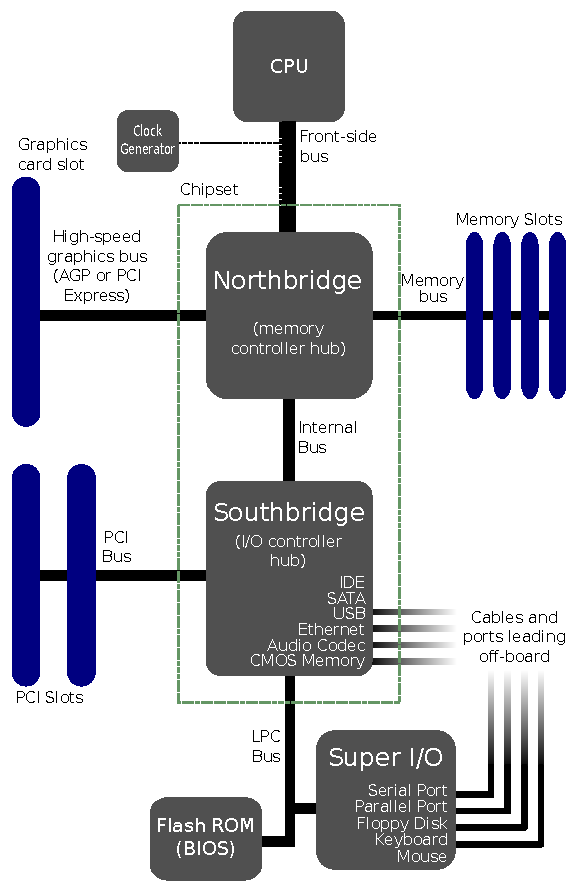
\includegraphics[width=0.38\textwidth]{figs/motherboard_diagram.pdf}
	\caption{现代计算机系统架构\cite{wiki:mb-fig}}
	\label{fig:mb-diag}
\end{figure}

可见中央处理器通过前端总线(Front-Side Bus,FSB)与北桥相联,北桥中包含PCIe
根集合体(Root Complex,RC)和DRAM存储器控制器,南桥向上通过内部总线(Internal Bus)
与北桥相联,向下提供多种中低速接口用于连接输入输出设备。

\section{SiFive Freedom U740 SoC结构简介}{Structure of the SiFive Freedom U740 SoC}
Freedom U740 SoC是SiFive公司于2021年推出的一款包含RISC-V处理器的片上系统,
这款SoC采用了多核异构架构,包含4个U系列核心和1个S系列核心,支持运行Linux操作系统。
搭载了U740 SoC的开发板名称为HiFive Unmatched,其上配备了16G DDR4 DRAM存储器,
以及PCIe、USB和千兆以太网等多种接口。

\begin{figure}[ht]
	\centering
	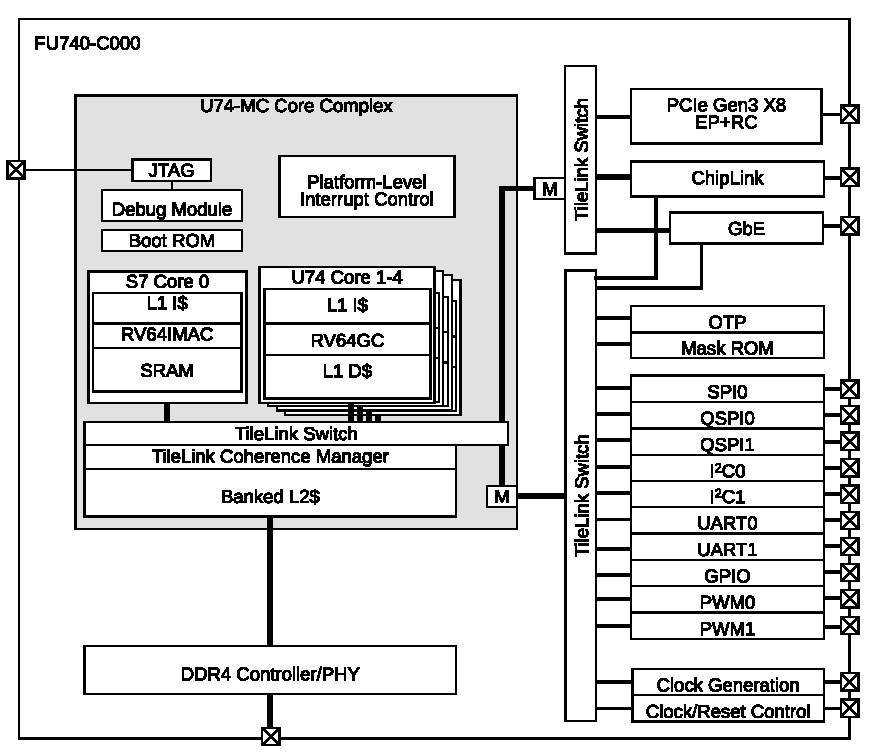
\includegraphics[width=0.8\textwidth]{figs/u740.pdf}
	\caption{U740 SoC架构\cite{noauthor_hifive_nodate}}
	\label{fig:u740}
\end{figure}

如图\ref{fig:u740}所示是Freedom U740 SoC的架构图,可见U740 SoC主要由处理器核
集合体(Core Complex)、高速外设(PCIe、ChipLink和千兆以太网)、低速外设(SPI、
UART和GPIO等)以及DDR4 DRAM存储器控制器四个部分组成,各部件间使用TileLink片上
总线相联。

\subsection{片上总线系统}{On-Chip Bus System}
Freedom U740 SoC上的处理器、存储器控制器以及各种外设通过高速片上总线和总线互联
相连接。片上总线承担了数据传输、数据一致性管理及时钟分配等功能。U740中由SiFive
公司自研的IP之间的连接采用TileLink总线协议,而DDR4存储器控制器、千兆以太网控制器
和PCIe根集合体等商用IP与系统其他部分的连接则采用AXI4总线协议。在TileLink总线与
AXI4总线间,插入了TL2AXI及AXI2TL双向协议转换器。整体片上总线系统(高速部分)结构
如图\ref{fig:u740-bus}所示。

\begin{figure}[ht]
	\centering
	\includegraphics[scale=1, page=4]{figs/figs.pdf}
	\caption{U740 SoC片上总线(高速部分)结构示意}
	\label{fig:u740-bus}
\end{figure}

可见PCIe设备可以通过以下数据路径访问DRAM存储器中的数据:PCIe根集合体
\rightarrow AXI2TL协议转换器 \rightarrow TileLink中央互联 \rightarrow
一致性管理器 \rightarrow 存储器控制器,如图\ref{fig:u740-bus}中的虚线箭头所示。
PCIe进行此类访问时无需处理器核的介入,从另一方面来说,处理器核
及运行在其上的程序无法控制,也无从得知PCIe设备正在访问DRAM存储器中的数据。

\subsection{PCIe 子系统}{PCIe Subsystem}
HiFive Unmatched开发板的PCIe子系统是由位于U740 SoC芯片内的PCIe根集合体、位于开发板
上的PCIe数据包交换机(Packet Switch)以及各种PCIe Endpoint设备所构成的。

\begin{figure}[ht]
	\centering
	\includegraphics[scale=1, page=5]{figs/figs.pdf}
	\caption{PCIe子系统结构}
	\label{fig:unmatched-pcie}
\end{figure}

如图\ref{fig:unmatched-pcie}所示是HiFive Unmatched开发板的PCIe子系统结构图,
稍后用于实现PCIe DMA攻击的FPGA开发板将会通过PCIe x16连接器接入U740 SoC。

\section{攻击方案}{DMA-Based Attack}
在2005年,\citet{becher2005firewire}展示了一种通过FireWire总线使用特制的
硬件实现了对计算机存储器的任意读写攻击。这一漏洞利用了FireWire总线使用的OHCI
(Open Host Controller Interface,开放主机控制器接口)协议的DMA功能。
值得注意的是OHCI提供了安全机制过滤从不可信外部设备传来的DMA请求,但当时很多
操作系统和驱动程序作者并没有运用这一安全机制。这一漏洞被发现后,主流操作系统均
启用了OHCI DMA请求过滤功能。

PCIe协议同样支持DMA传输,但PCIe协议本身并未提供任何用于过滤DMA请求的机制,
并且随着技术的进步,PCIe由于其传输速率高、使用信号数量少的特点,应用场景已经
不限于机箱内部扩展卡与主板间的连接,而是通过雷电(Thunderbolt)、USB4等接口
协议用于连接外部设备,所以基于PCIe的DMA攻击成本将越来越低。

本章将使用Xilinx KCU116 FPGA开发板实现一个软件可控的PCIe Endpoint设备,
将其连接到HiFive Unmatched开发板的PCIe子系统中,使用PCIe DMA功能实现
对一处运行在U740 SoC上Linux操作系统中程序的秘密信息的读取。


\section{可行性验证}{An Attack Example Based on PCIe DMA}
\subsection{可控PCIe Endpoint实现}{Implementation of PCIe Endpoint}
本小结将实现一个软件可控的PCIe Endpoint设备,可以将上位机下发的读写命令
转换成PCIe传输事务(Transaction)发送给PCIe上游设备,并将收到的响应内容回传
给上位机程序。

由于PCIe协议复杂,Xilinx的FPGA系列中均包含专有硬件实现的PCIe控制器,本设计
使用的KCU116开发板上搭载的FPGA型号为XCKU5P,属于Kintex UltraScale+产品线,
也内置了PCIe控制器\cite{pg213}。PCIe硬件控制器与用户逻辑交互的接口AXI Stream
流式传输接口,其上传输的数据为PCIe TLP(Transaction Layer Packet,事务层数据包),
较难处理。于是本设计使用Xilinx提供的PCIe AXI桥IP实现AXI传输事务与PCIe传输事务
的相互转换。在上位机控制方面,本设计采用JTAG2AXI IP,通过JTAG调试接口接收上位机
的读写命令,并转换成AXI传输事务送入PCIe AXI桥,从而实现从上位机命令到PCIe传输事务
及的转换。在相反方向上,从外部PCIe接口传入的数据读取响应被PCIe AXI桥转换成AXI读响应,
由JTAG2AXI IP通过JTAG接口回传给上位机。如图\ref{fig:pcie-ep}所示是
PCIe Endpoint的结构简图。

\begin{figure}[ht]
	\centering
	\includegraphics[scale=1, page=6]{figs/figs.pdf}
	\caption{PCIe Endpoint的结构}
	\label{fig:pcie-ep}
\end{figure}

完整的软件可控PCIe Endpoint在Vivado软件中的实现在附录\ref{app:pcie-ep}中。

\subsection{Linux 物理地址获取}{Acquisition of Physical Address on Linux}
Linux操作系统及其上运行的所有程序均运行在各自的虚拟存储器地址空间中,处理器发起的
每个对存储器的访问请求均使用虚拟地址寻址,由MMU根据页表(Page Table)将虚拟地址
翻译成物理地址后用于寻址DRAM存储器。但PCIe子系统访问DRAM存储器直接使用便的是物理
地址,要想通过PCIe Endpoint设备访问Linux系统中运行着的程序数据,就需要将程序使用
的虚拟地址翻译成物理地址。

在Linux操作系统中,出于安全考虑,禁止在非特权用户态获取其他进程或内核虚拟地址对应
的物理地址(禁止读取非当前进程的页表),但仍然有很多安全漏洞可以使攻击者在非特权
情况下完成地址翻译\cite{chen2011linux}。并且考虑到所有进程的页表都存储在DRAM存储器
中,而本文介绍的PCIe DMA攻击可以读取任意DRAM存储器地址,所以完全可以通过使用PCIe DMA
攻击方案读取任意进程的页表以实现地址翻译。但由于地址翻译不是本文的主要内容,此处
使用更加简便的使用特权账户执行软件读取内核数据结构的方式完成地址翻译。

\begin{table}[!ht]
	\centering
\begin{threeparttable}[b]
\zihao{5}
\caption{pagemap文件页表项结构}
\begin{tabular}{x{0.2\textwidth}x{0.4\textwidth}}
	\toprule
	位域 & 含义 \\
	\midrule
	0-54 & 物理页号(Page Frame Number,PFN) \\
	55 & 页表项脏(PTE Dirty) \\
	56 & 页被独占映射 \\
	57-60 & 全为零 \\
	61 & 页是文件页或共享匿名页 \\
	62 & 页被换出(Swapped) \\
	63 & 页存在 \\
	\bottomrule
\end{tabular}
\label{tab:pagemap-entry}
\end{threeparttable}
\end{table}

Linux内核通过/proc/<pid>/pagemap特殊文件向用户空间暴露出进程号为pid的进程的页表
所对应的内核数据结构。在这一文件中,每一个虚拟地址页都对应一个64位长的数据结构,
称之为pagemap项(Entry),每一项的结构及其含义在表\ref{tab:pagemap-entry}中列出。
整个虚拟地址空间中所有可能的虚拟地址页(包括暂未被映射的页)的pagemap项被按虚拟地址
页号顺序存放在pagemap文件中。\cite{pagemap}

所以在Linux系统中使用pagemap特殊文件将进程号为$p$的的进程中,虚拟地址$v$翻译成
物理地址的过程可以描述为如下步骤:
\begin{compactenum}
	\item 打开/proc/$p$/pagemap文件;
	\item 根据虚拟地址$v$算出虚拟页号$v / \text{PAGE\_SIZE}$;
	\item 根据虚拟页号求得pagemap项在pagemap文件中的偏移地址;
	\item 从求得的偏移地址中读取pagemap项;
	\item 根据pagemap项中的物理页号将虚拟地址翻译为物理地址。
\end{compactenum}

附录\ref{app:v2p}记载了使用上述方法实现从虚拟内存地址到物理内存地址翻译
的C源程序。本攻击后续将使用附录\ref{app:v2p}中的程序完成虚拟内存地址到物理内存地址
的翻译。

\subsection{秘密信息读取}{Readout of Secret Data}

\begin{figure}[ht]
	\centering
	\begin{lstlisting}[language=c, escapechar=|]
#include <stdio.h>
#include <unistd.h>
char secret[128];
int main() {
	fprintf(stderr, "%d %p\n", getpid(), secret);
	gets(secret);
	while (1) puts(secret);
	return 0;
}
	\end{lstlisting}
	\caption{被攻击程序源代码}
	\label{fig:target-src}
\end{figure}

将软件可控PCIe Endpoint综合实现后载入FPGA中,并将KCU116开发板通过PCIe x16插槽与
HiFive Unmatched开发板连接后,启动两块开发板。进入Linux操作系统后,首先运行命令:

setpci -s 07:00.0 COMMAND=6

\noindent 使能PCIe Endpoint总线主设备功能。接着编译如图\ref{fig:target-src}
所示的测试程序作为被攻击的对象。测试程序从命令行参数接收一个用户指定的字符串,存入
secret指向的存储器地址中,并打印出自身的进程号和secret的虚拟地址,本例中使用Hellp
作为secret字符串,得到进程号和地址分别为687和0x2ab5ee8078。
接着运行附录\ref{app:v2p}中的地址翻译程序,将测试程序打印出的
进程号和虚拟地址作为参数传入,可得到对应的物理地址为0x10689d078。图\ref{fig:unmatched-output}为上述命令
在Linux系统中的运行结果。

\begin{figure}[ht]
	\centering
	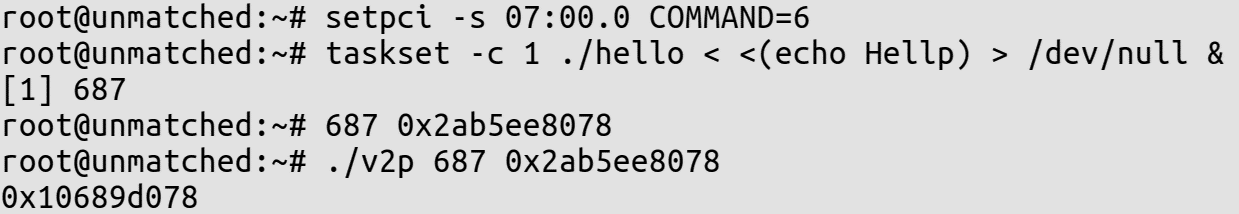
\includegraphics[width=0.7\textwidth]{figs/unmatched.png}
	\caption{Linux被攻击程序运行结果}
	\label{fig:unmatched-output}
\end{figure}

攻击者只需在通过JTAG调试接口连接FPGA的上位机Vivado软件中运行TCL命令:

\verb|create_hw_axi_txn rd0 [get_hw_axis hw_axi_2] -address 10689d078 \|

\verb|    -len 1 -type read -f|

\verb|run_hw_axi rd0|

\noindent 生成并执行一个对地址10689d078的读取命令,得到返回值为:000000706c6c6548,
如图\ref{fig:vivado-output}所示,
与最初指定的secret字符串的ASCII值H(0x48) e(0x65) l(0x6c) l(0x6c) p(0x70)一致,
可以证明攻击成功,实现了对Linux操作系统中程序的秘密信息的读取,并且只要更换
PCIe DMA指令的地址,就可以实现对任意存储器地址的访问。

\begin{figure}[ht]
	\centering
	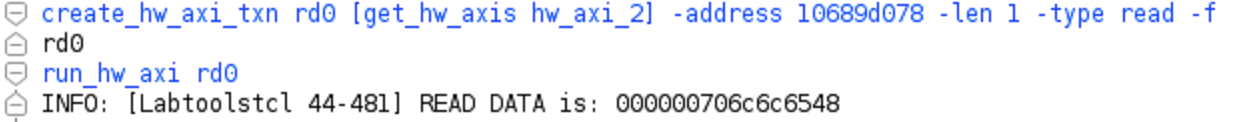
\includegraphics[width=0.85\textwidth]{figs/vivado.png}
	\caption{控制PCIe Endpoint读取DRAM的结果}
	\label{fig:vivado-output}
\end{figure}

\section{本章小结}{Chapter Summary}
本章首先介绍了现代计算机系统的常见架构:处理器、存储器和输入输出设备通过总线相连,
各部件可以通过总线与其他部件通信。

随后展开介绍了用于攻击方案演示的HiFive Unmatched开发板上的PCIe子系统以及U740 SoC
的片上总线系统结构,论证了PCIe Endpoint通过PCIe DMA机制访问DRAM存储器的可行性,并
给出了DMA访问的数据路径。

接着介绍了基于PCIe DMA的任意存储器地址访问攻击方案的整体思路,并与前人提出的其他
DMA攻击方案做了对比。

最后通过在FPGA上设计可控PCIe Endpoint,并解决了Linux系统下虚拟地址到物理地址的
翻译问题,从而在HiFive Unmatched硬件上实现了基于PCIe DMA的任意存储器地址访问攻击。


\newpage
